% APENDICE A
\chapter{Roteiro de Entrevista}
\label{ap:entrevista}

\vspace{4mm}

\textbf{Introdução}

Esta entrevista faz parte de uma pesquisa de trabalho de graduação do pesquisador Geraldo Pereira sob a orientação do professor Kiev Gama da Universidade Federal de Pernambuco (UFPE). O objetivo é comprovar a ciência dos participantes de Hackathons sobre seus direitos à Propriedade Intelectual e suas motivações para cederem ou não tal direito. Na entrevista, procuramos entender aspectos motivacionais e percepção dos participantes de hackathons sobre o assunto.
Todas as informações fornecidas nesta entrevista serão tratadas de forma confidencial. Apenas a equipe de pesquisa terá acesso às informaões fornecidas. 
Não existem respostas corretas, seus dados são confidenciais e não serão divulgados. O intuito é extrair sua opinião a fim de contribuir para um estudo do momento atual das organizações de eventos a respeito do tema.

Sua participação nesta pesquisa é voluntária e você pode decidir por não participar ou retirar-se da pesquisa a qualquer momento. Caso você decida pela não participação, não receberá sanções ou penalidades.

Você concorda em participar desta pesquisa?

(Iniciar a gravação do áudio)
Você autoriza a gravação desta entrevista?
\vspace{4mm}

\textbf{Questões}

\textit{Dados demográficos:}

Formação:

Cargo do entrevistado(a):

Idade do entrevistado(a):

Gênero:

Naturalidade:

\vspace{4mm}
\textit{Questões sobre hackathons}

Quantidade de Hackathons realizadas:

Onde trabalha/estuda, já participou de eventos de Hackathons? 

Qual a sua motivação para participar de Hackathons?

Qual evento e o tipo de hackathon que você participou iremos abordar?
Exemplo dos tipos: Governamental, Empresarial, Recrutamento de Talentos, Criação de Novas Soluções (Melhorias na Sociedade)

\vspace{4mm} 
\textit{Questões sobre Propriedade Intelectual x Hackathon}

O que você entende por Propriedade Intelectual?

Qual a sua percepção sobre a importância (o quão importante é para você o assunto de PI na Hackathon) e o nível de prioridade dado pela organização do evento com relação aos direitos sobre propriedade intelectual?

Numa hackathon, o que você considera como prioridade ao ler o regulamento? Gostaria que enumerasse de 1 a 5 onde 1 é o mais importante e 5 o menos importante, dentre os seguintes critérios; Critério de avaliação, premiação, direitos à propriedade intelectual, organização da equipe, programação; (Se tiver outra prioridade pode acrescentar na lista e definir sua prioridade)

De acordo com o regulamento proposto, o quão claro fica  os direitos à propriedade intelectual do conteúdo feito por você naquele evento?

(Se participou de outros tipos) Conte também sobre os regulamentos de outros hackathons que participou e a clareza sobre os direitos à propriedade intelectual.

Quando participa de um evento de hackathon, o que você sente a respeito do seu direito a propriedade intelectual?

Venderia sua solução? Se sim, por quanto?

\vspace{4mm}
\textit{Para quem possui várias experiências em Hackathons}

Qual a principal diferença com relação a propriedade intelectual dentre as outras hackathons que participou? (Caso haja) Cite exemplos negativos.

\vspace{4mm}
\textit{Questões sobre Cessão de Direitos}

Deixaria de participar de uma hackathon caso o direito à propriedade intelectual não ficasse com você?

Tem confiança em ceder os códigos-fonte após o evento para a empresa organizadora?

Nos eventos, sente que seu direito à propriedade intelectual é respeitado?


\vspace{4mm}
\textit{Encerramento}

Há algo que você deseja acrescentar sobre este assunto?




%%%%%%%%%%%%%%%%%%%%%%%%%%%%%%%%%%%%%%%%%%%%%%%%%%%%%%%%%%
%%%%%%%%%%%%%%%%%%%%%%%%%%%%%%%%%%%%%%%%%%%%%%%%%%%%%%%%%%

% APENDICE B
\chapter{Termo de Consentimento da Entrevista}
\label{ap:termoConcent}
\begin{minipage}{10cm}
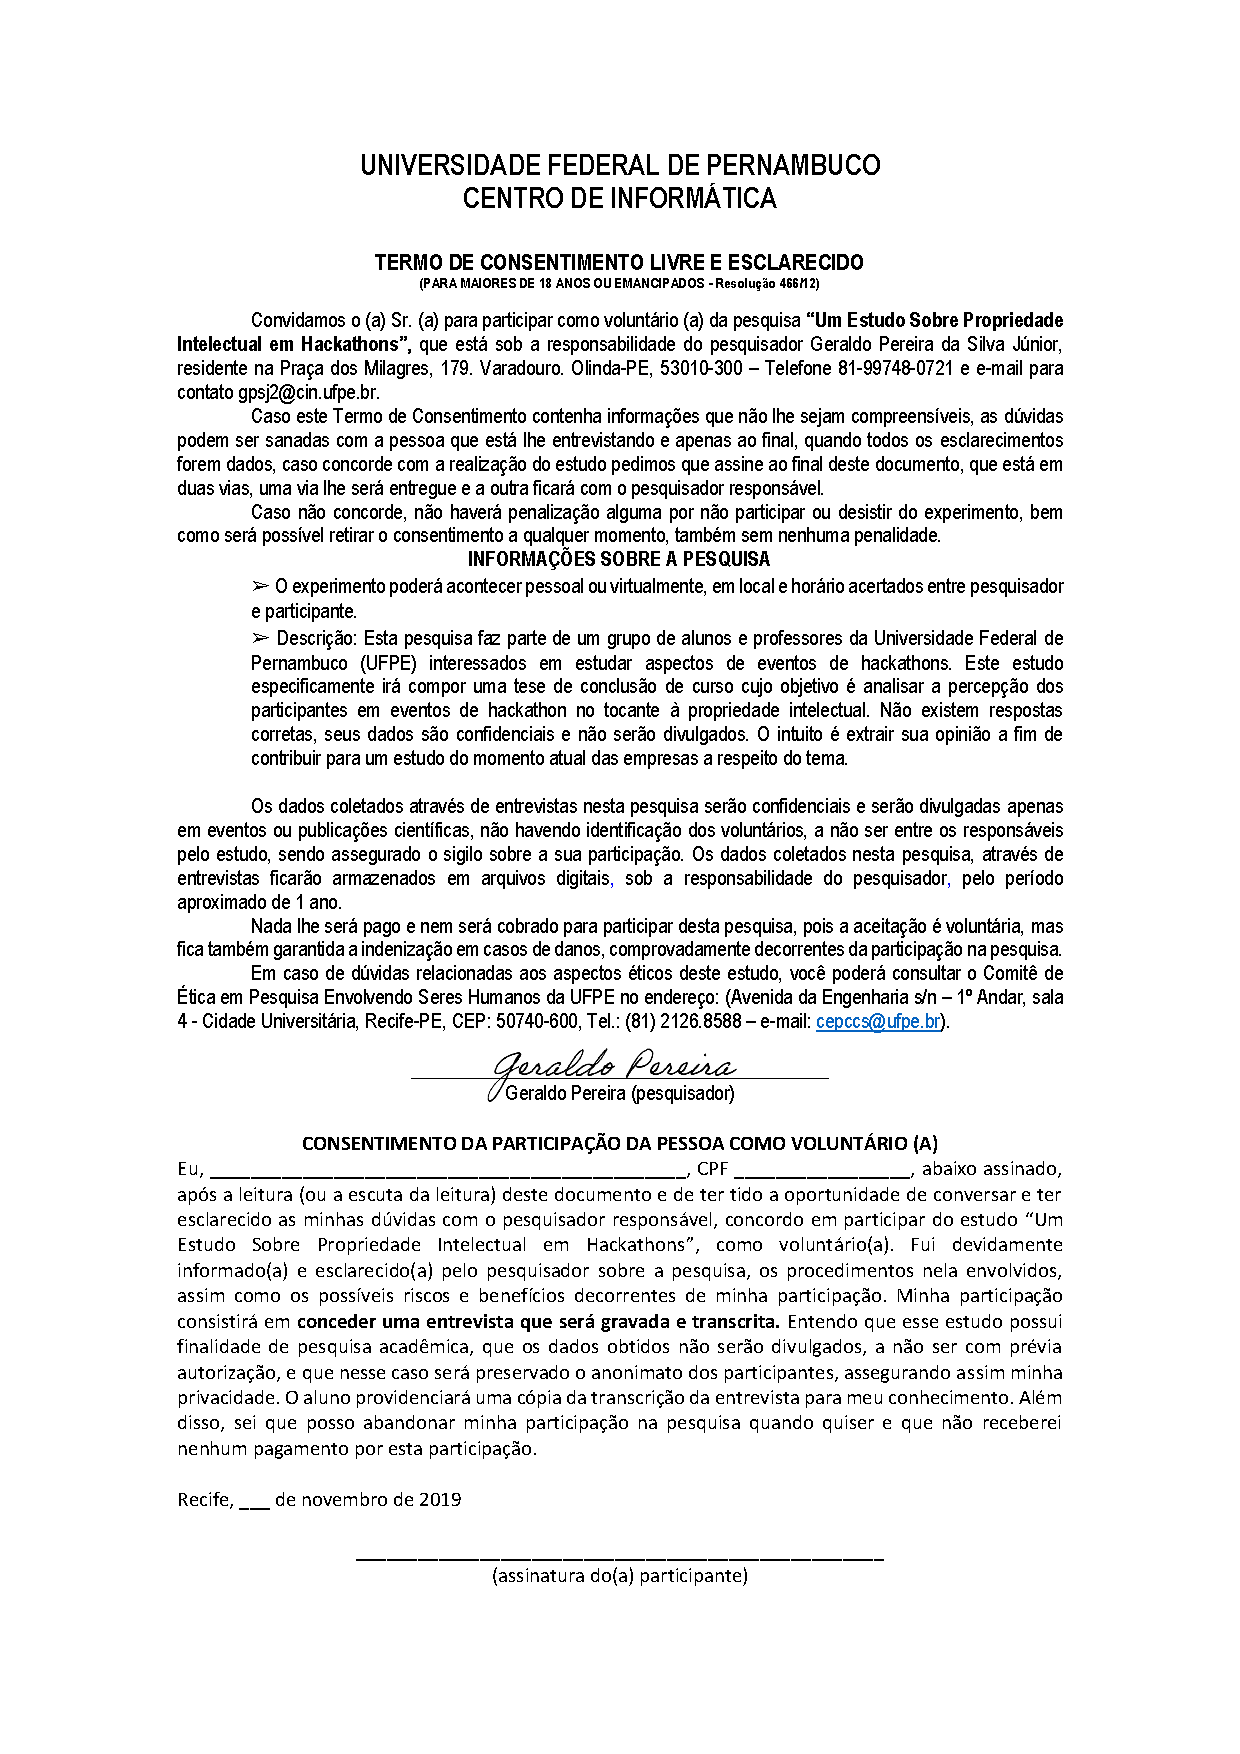
\includepdf[scale=0.80]{appendix/TermoConsentimento.pdf}
\end{minipage}
%%%%%%%%%%%%%%%%%%%%%%%%%%%%%%%%%%%%%%%%%%%%%%%%%%%%%%%%%%
%%%%%%%%%%%%%%%%%%%%%%%%%%%%%%%%%%%%%%%%%%%%%%%%%%%%%%%%%%

% APENDICE C

\chapter{Questionário}
\label{ap:questionario}
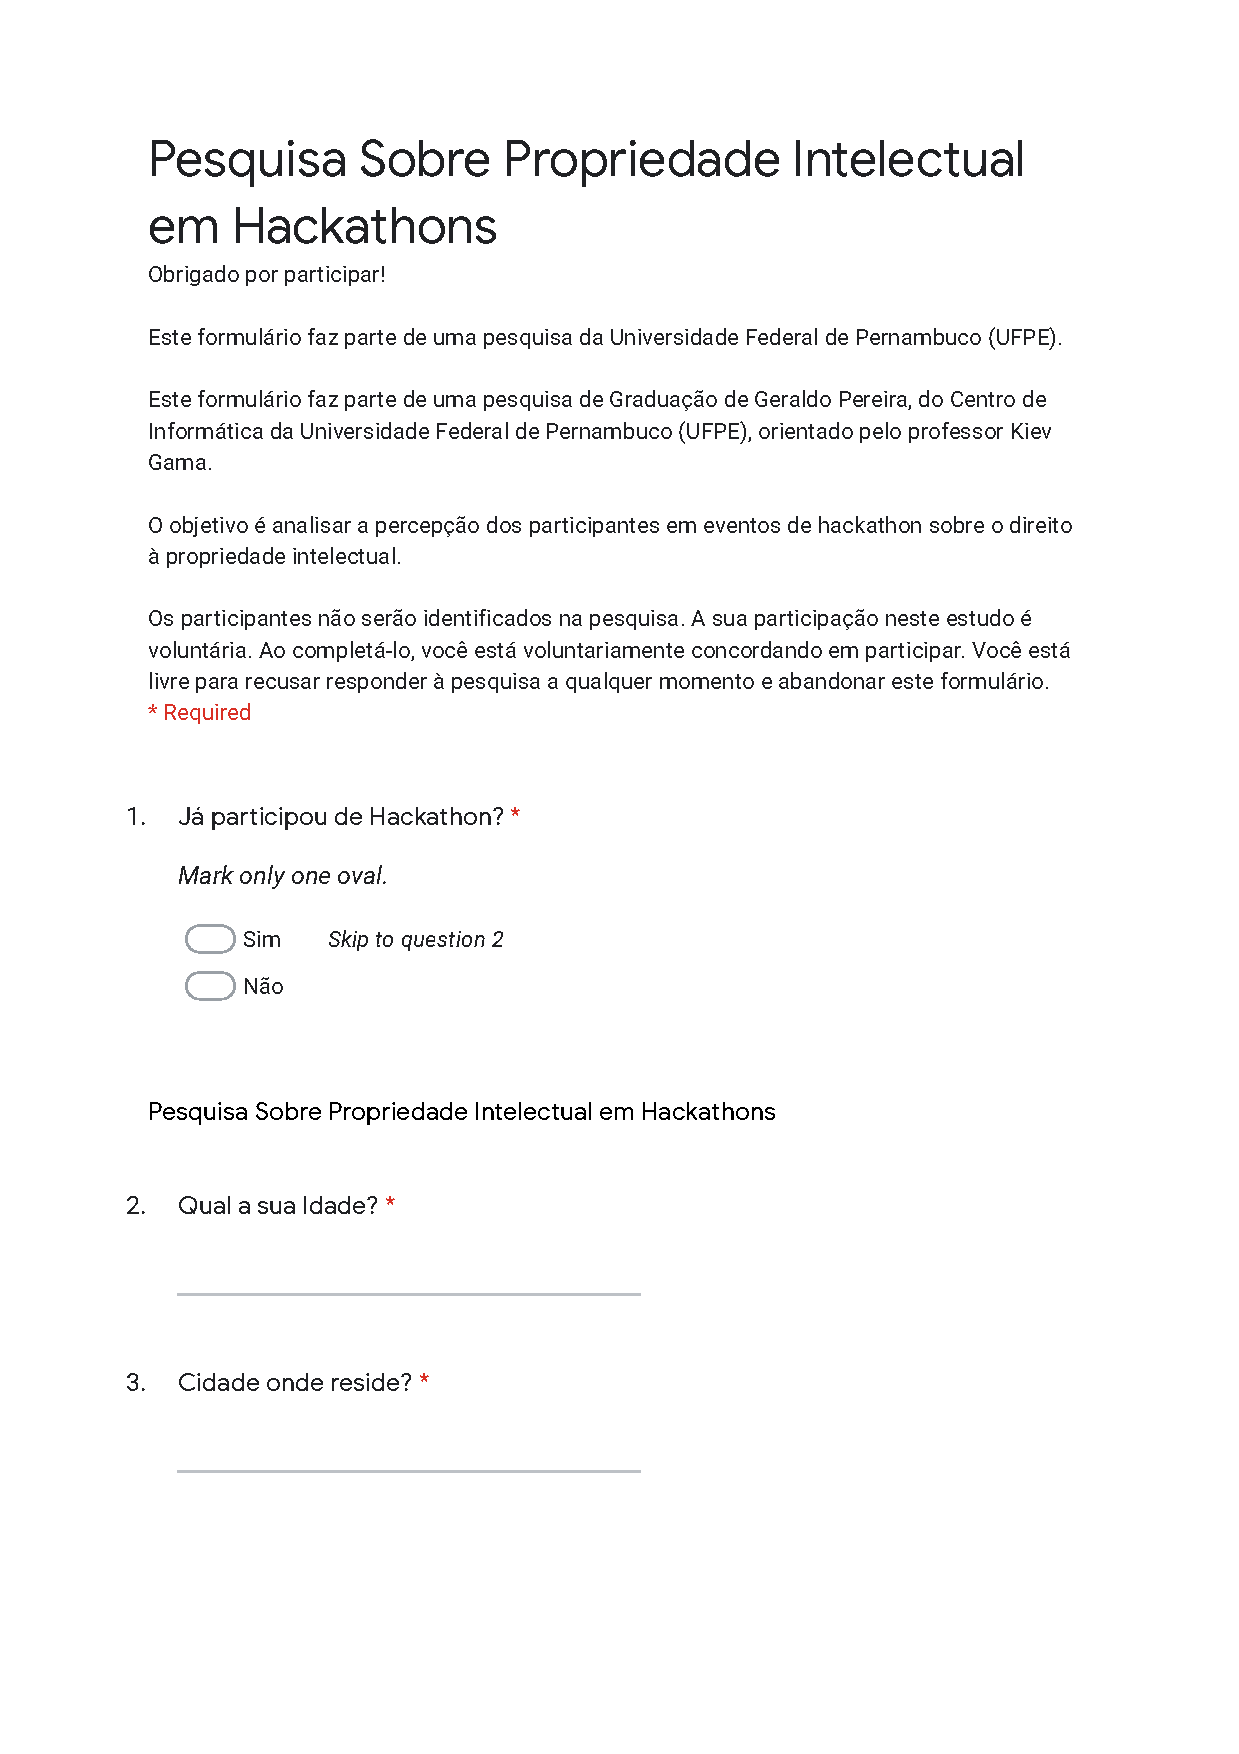
\includegraphics[scale=0.75]{appendix/FormularioGForm.pdf}

\includepdf[pages={2-6},width=\textwidth]{appendix/FormularioGForm.pdf}

%%%%%%%%%%%%%%%%%%%%%%%%%%%%%%%%%%%%%%%%%%%%%%%%%%%%%%%%%%
%%%%%%%%%%%%%%%%%%%%%%%%%%%%%%%%%%%%%%%%%%%%%%%%%%%%%%%%%%

% APENDICE D

\chapter{Nuvem de Palavras}
\label{ap:nuvem}

\begin{figure}[H]
    \centering
    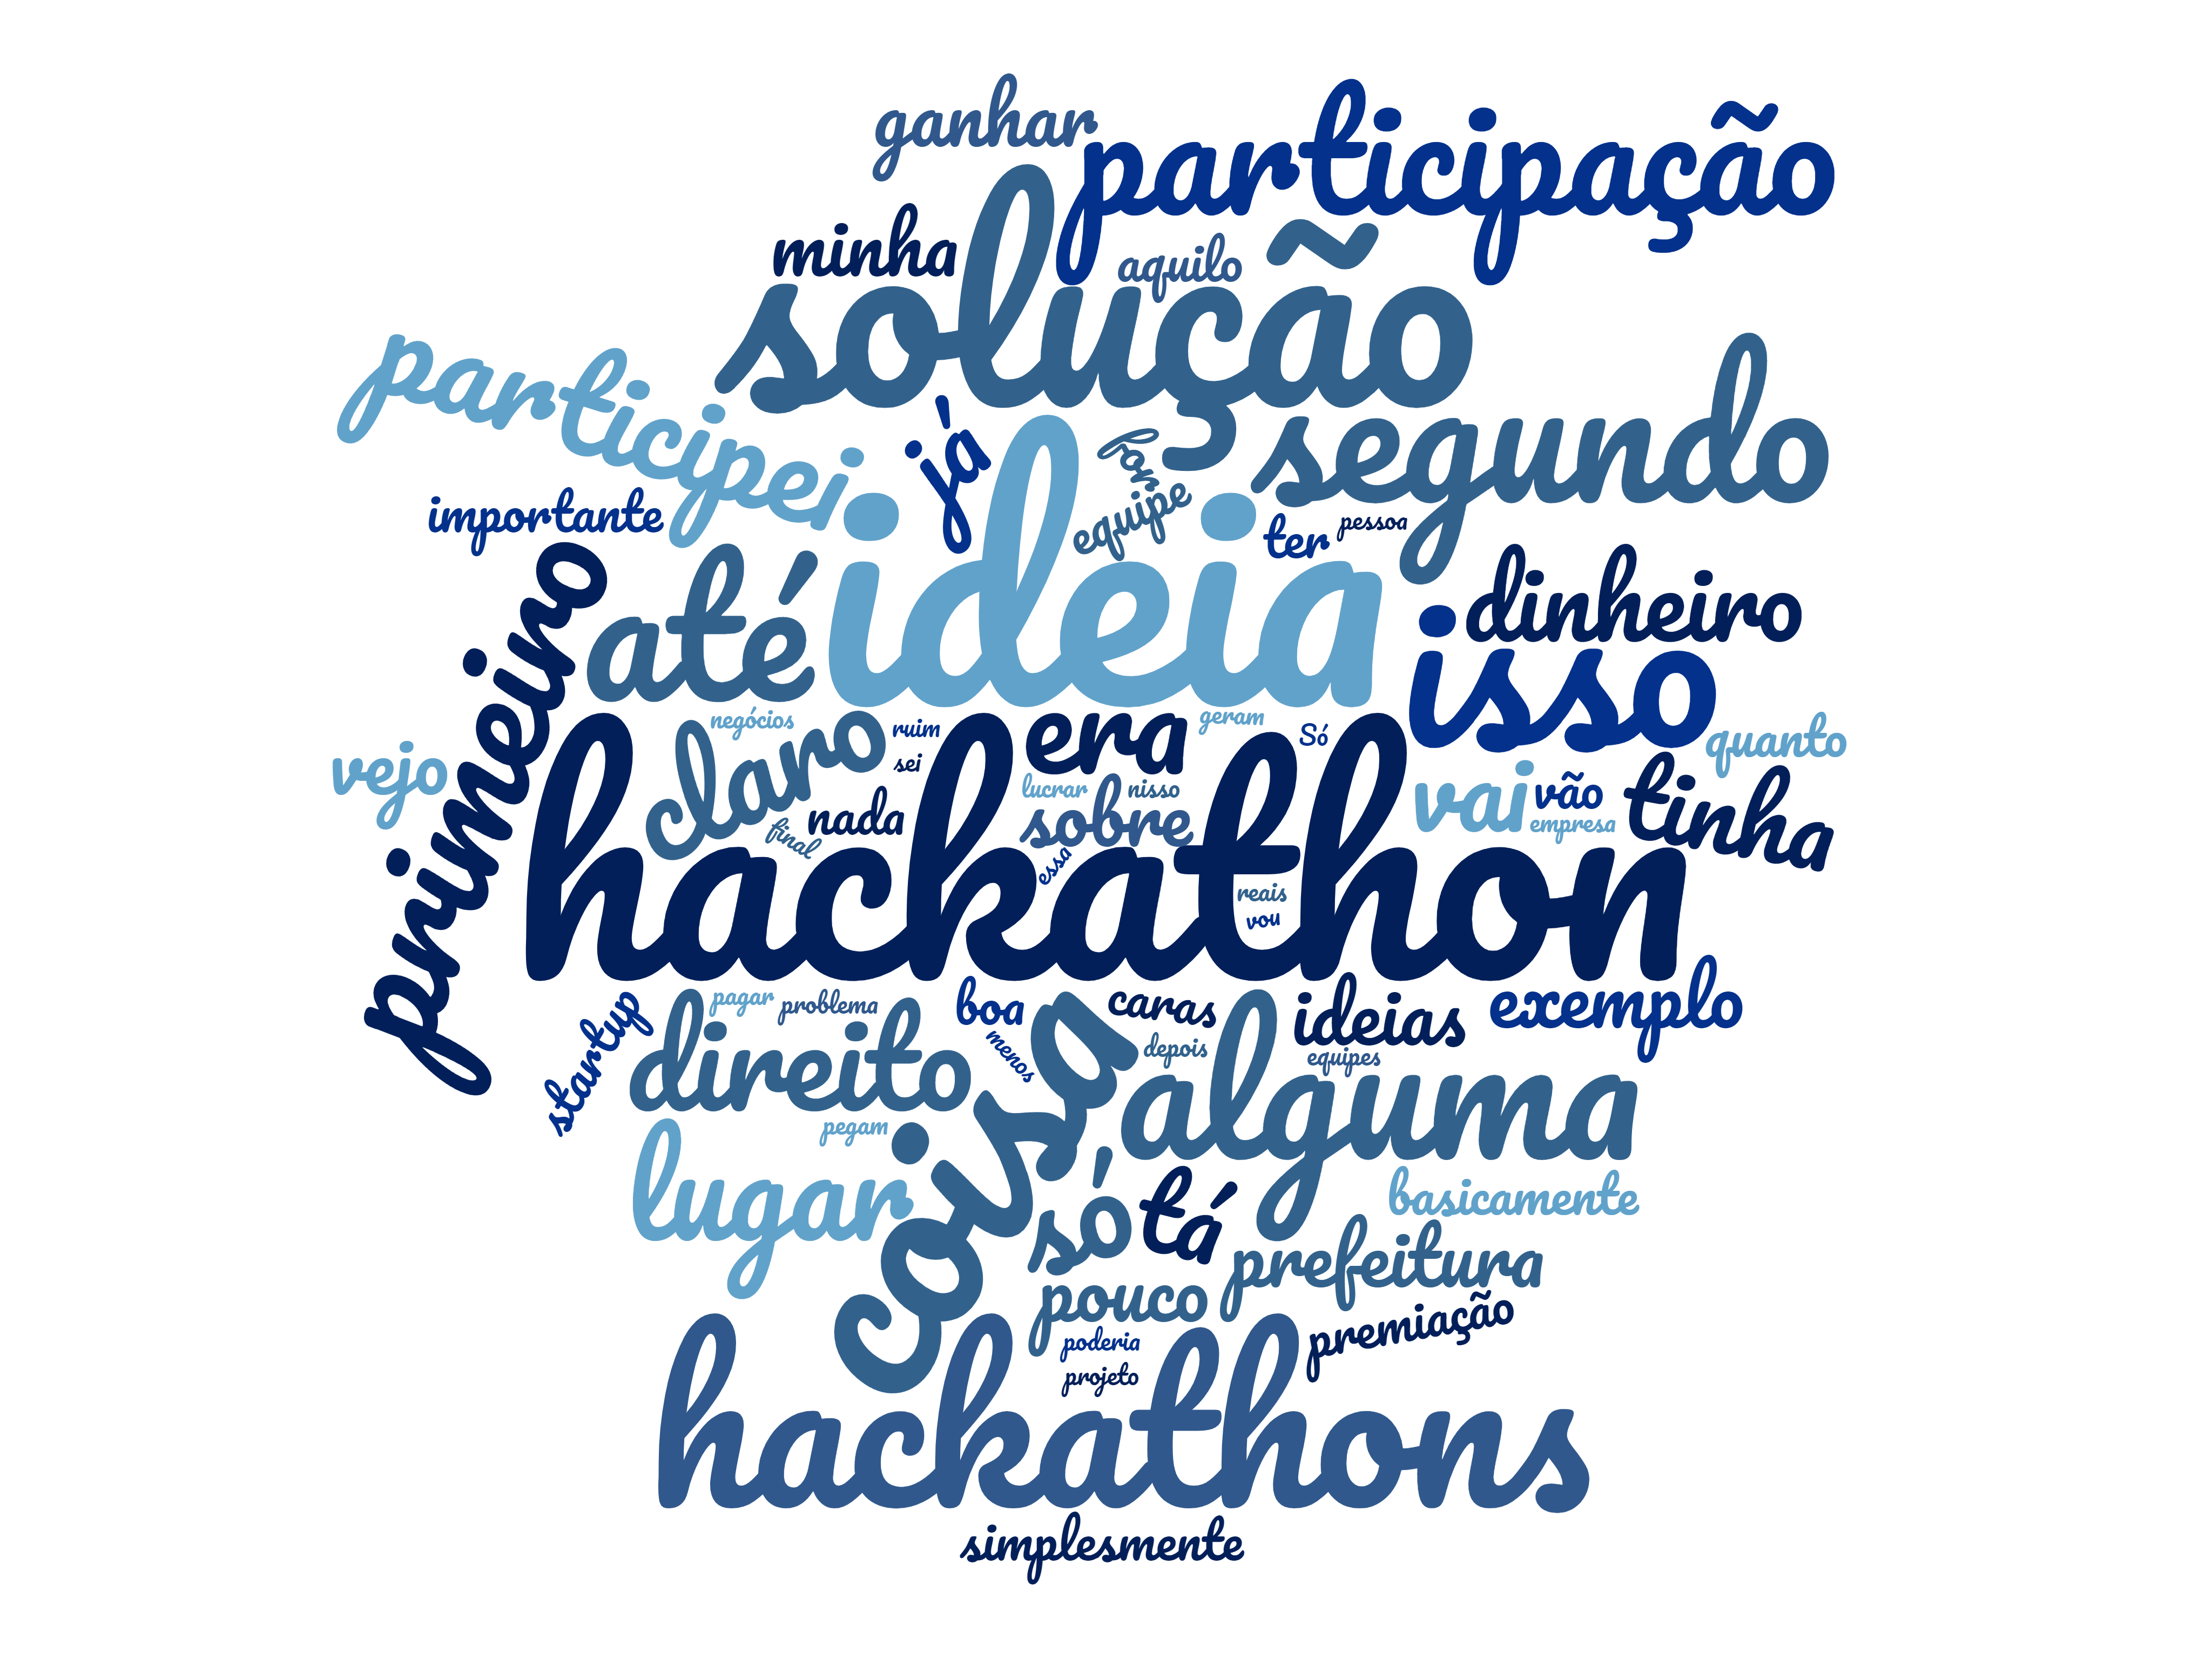
\includegraphics[width=0.7\textwidth]{appendix/wordcloud1.png}
    \caption{Nuvem de palavras do entrevistado 1}% nuvem 1
    \label{fig:nuvem-1}
\end{figure}

\begin{figure}[H]
    \centering
    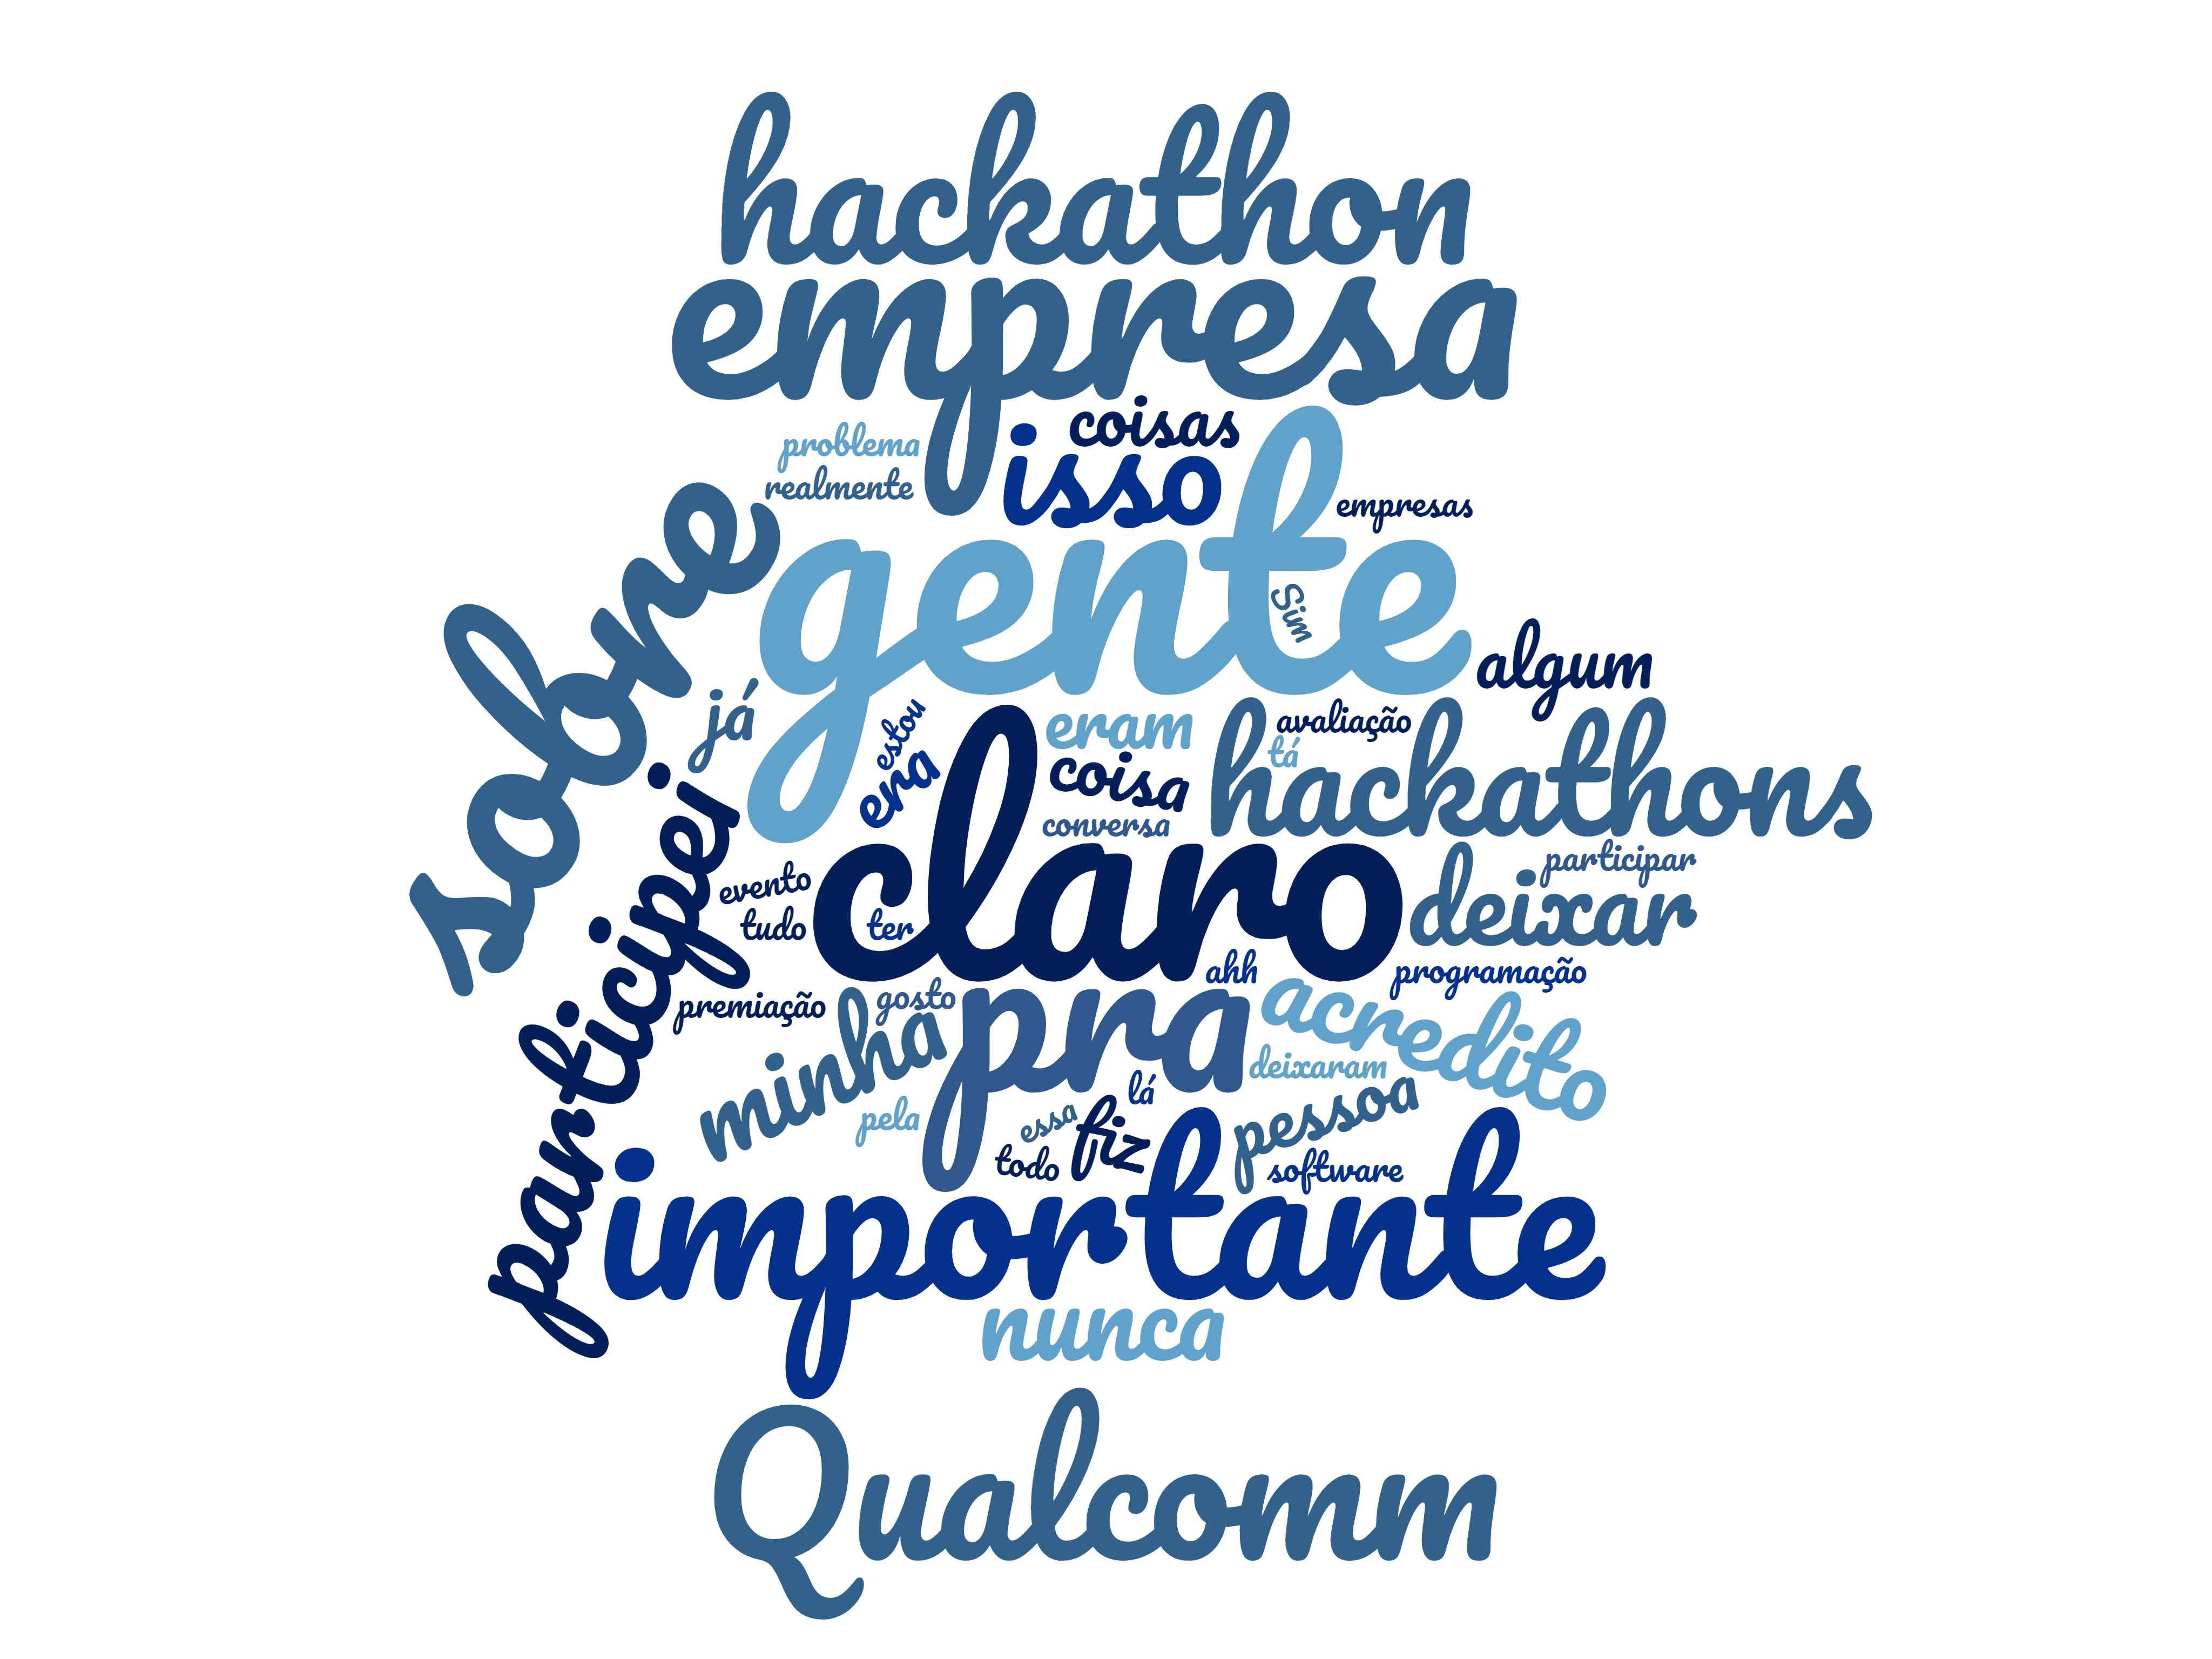
\includegraphics[width=0.7\textwidth]{appendix/wordcloud2.png}
    \caption{Nuvem de palavras do entrevistado 2}% nuvem 2
    \label{fig:nuvem-2}
\end{figure}

\begin{figure}[H]
    \centering
    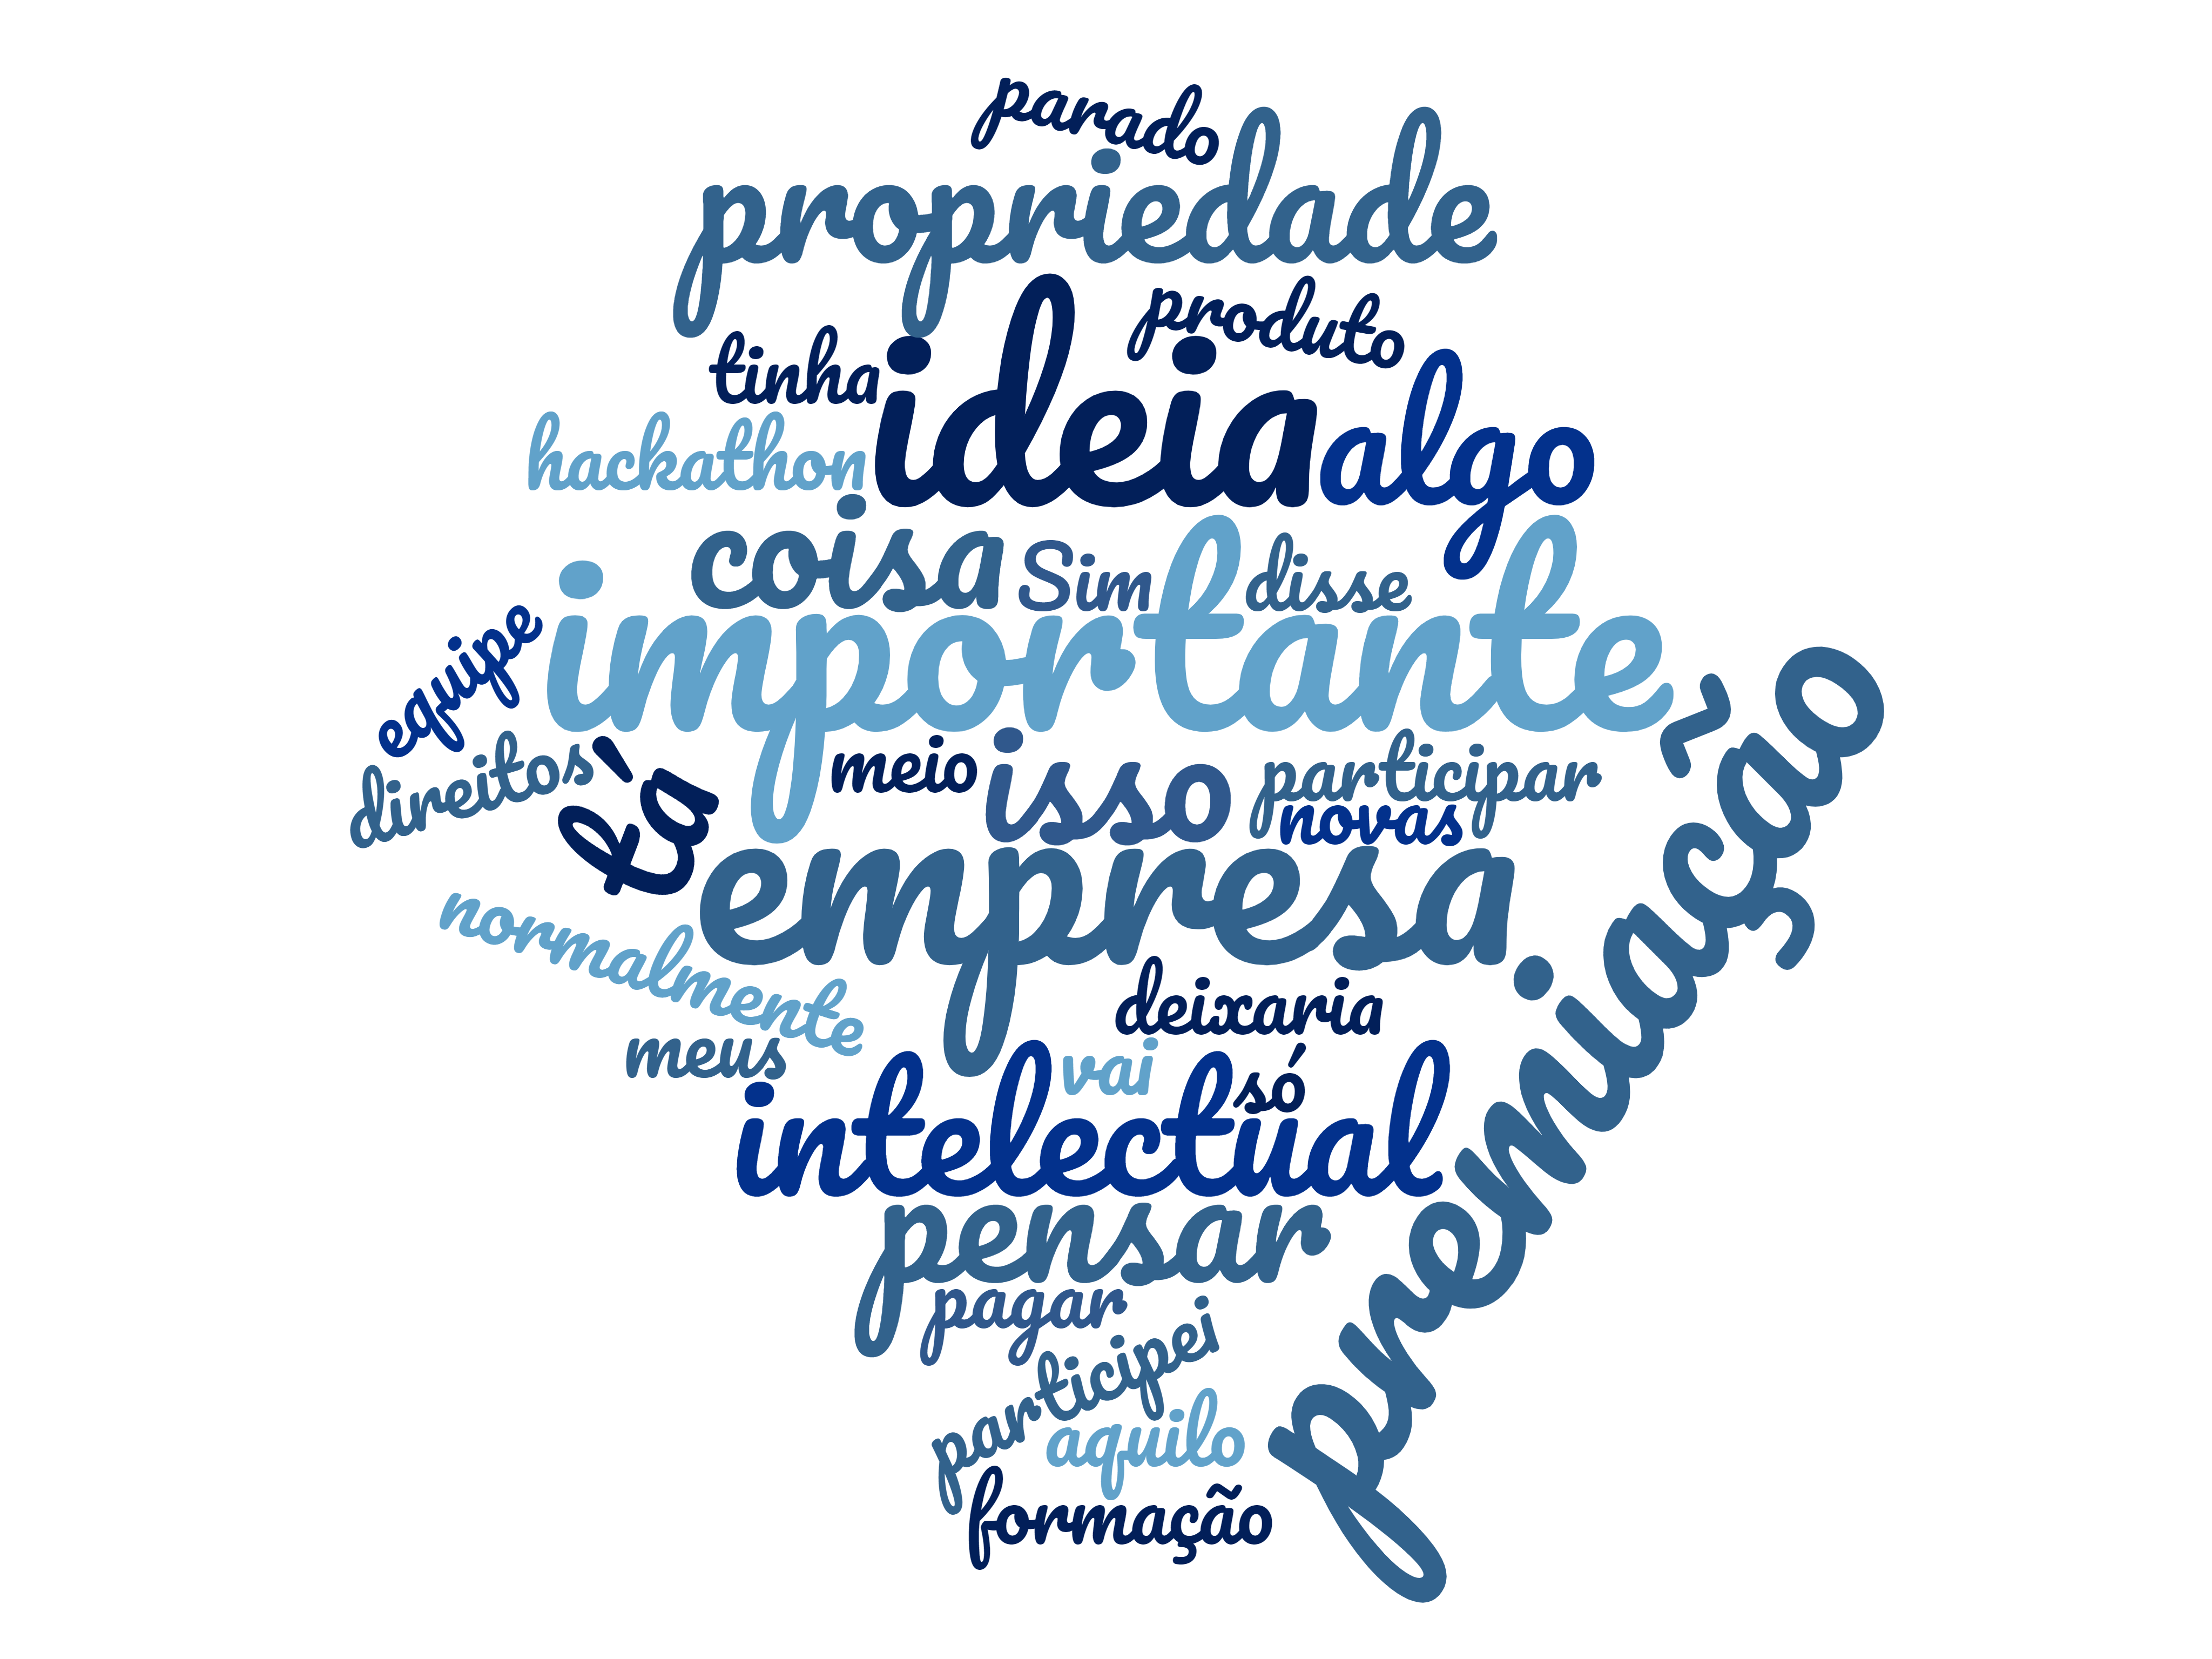
\includegraphics[width=0.7\textwidth]{appendix/wordcloud3.png}
    \caption{Nuvem de palavras do entrevistado 3}% nuvem 3
    \label{fig:nuvem-3}
\end{figure}

\begin{figure}[H]
    \centering
    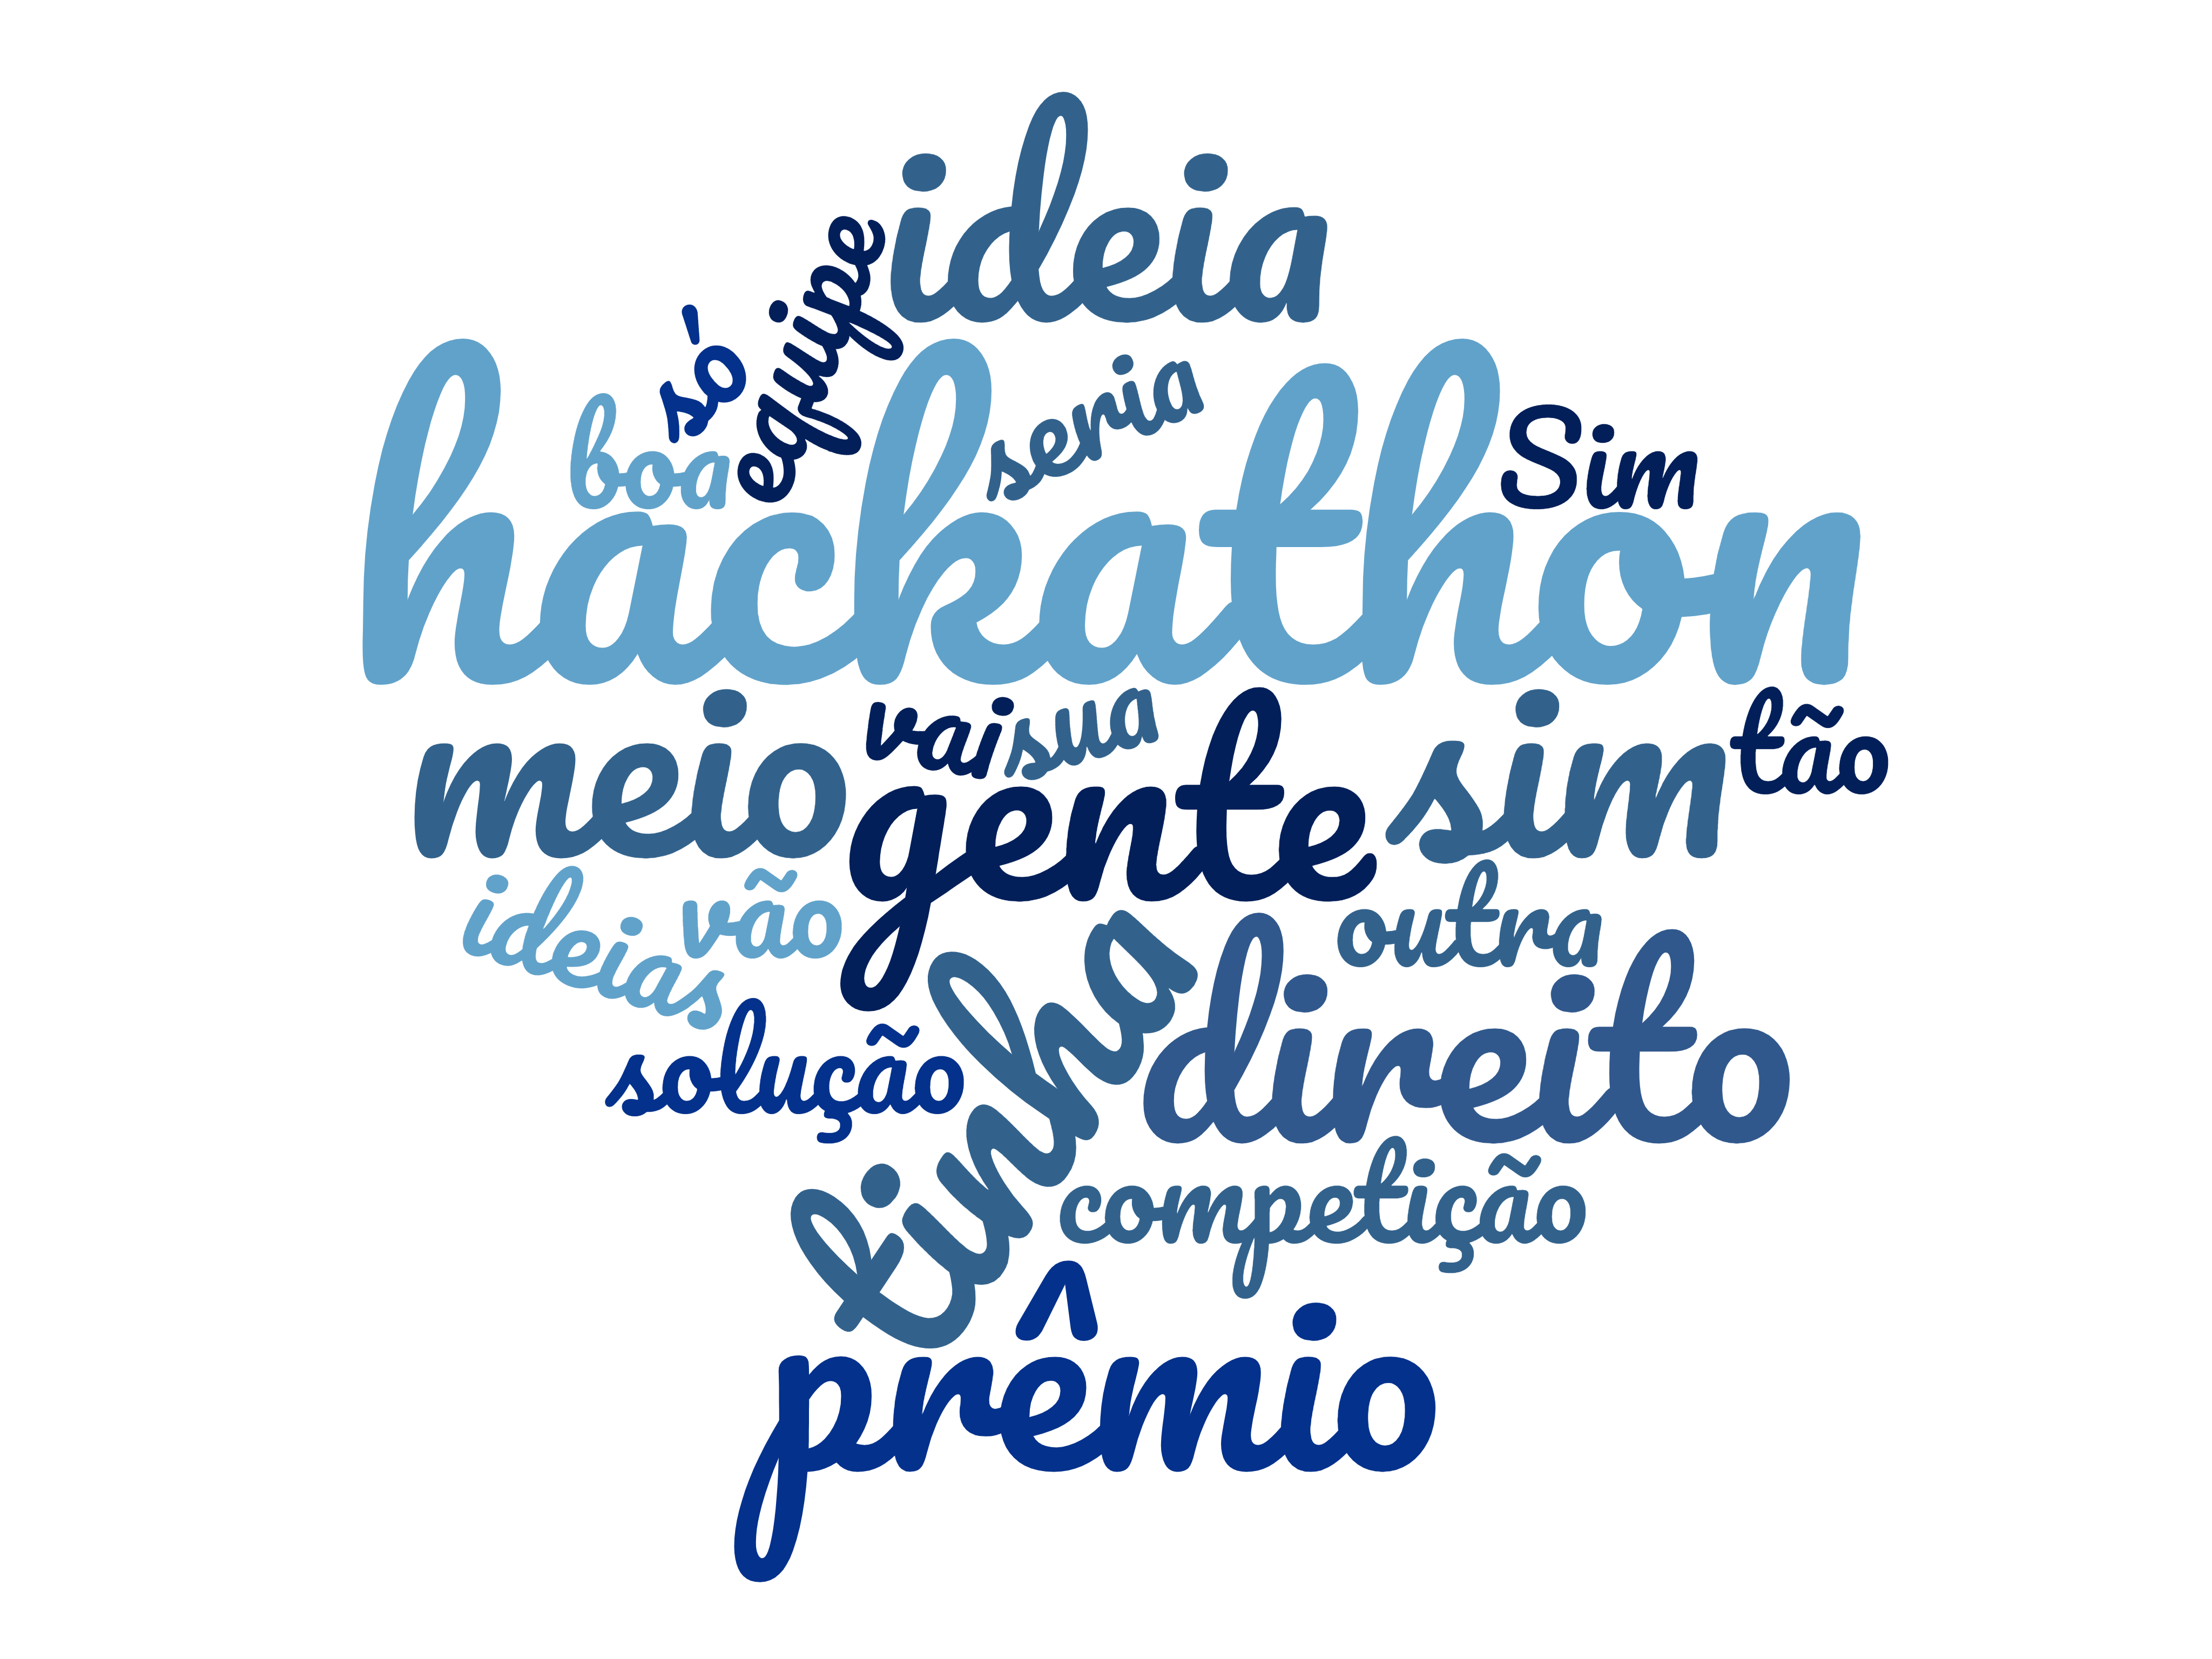
\includegraphics[width=0.7\textwidth]{appendix/wordcloud4.png}
    \caption{Nuvem de palavras do entrevistado 4}% nuvem 4
    \label{fig:nuvem-4}
\end{figure}

\begin{figure}[H]
    \centering
    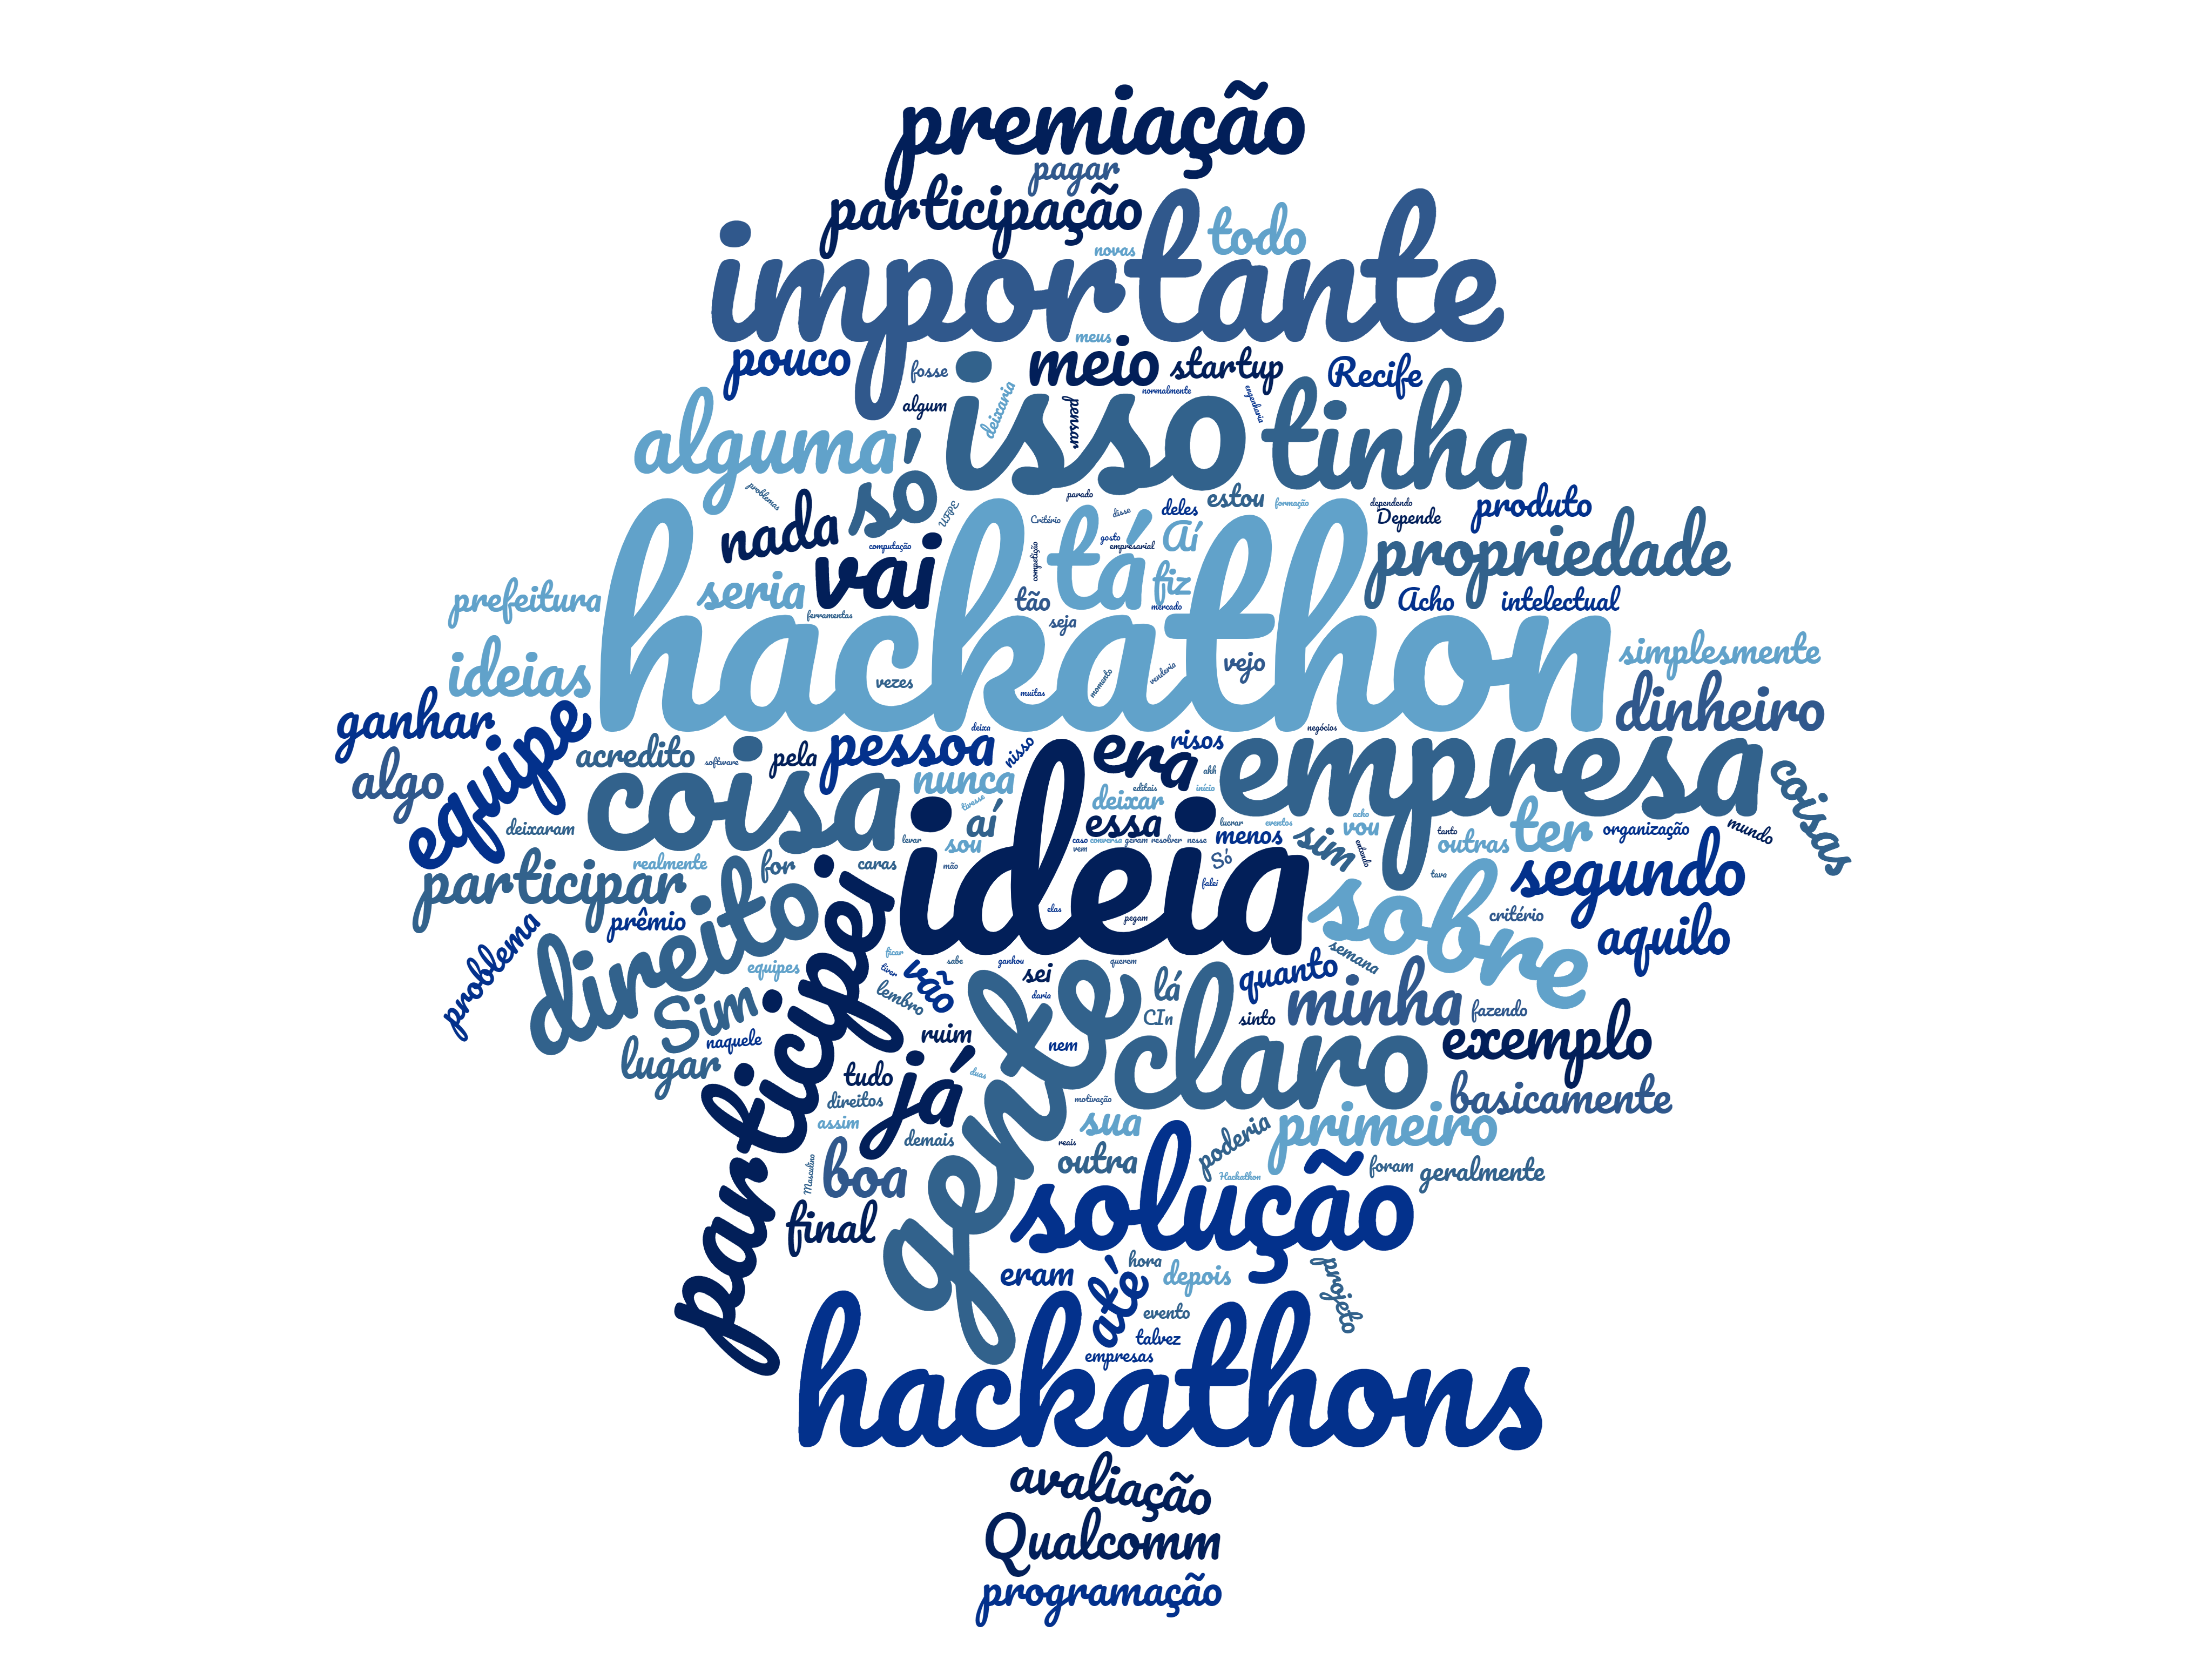
\includegraphics[width=1\textwidth]{appendix/wordcloudTODOS.png}
    \caption{Nuvem de palavras de todos os entrevistados}% nuvem geral
    \label{fig:nuvem-todos}
\end{figure}